\chapter{Automação}

\section{Definição dos itens da automação}

	Automação pode ser definida como um conjunto de técnicas que podem ser aplicadas sobre um processo objetivando torná-lo mais eficiente, ou seja, maximizando a produção com menor consumo, menor emissão de resíduos e melhores condições de segurança \cite{2009AutomacaoMarilia}.

	Com a finalidade de lançar no mercado um produto competitivo, as subrotinas e cômodos a serem automatizados foram definidos de acordo com os atuais sistemas empregados, de modo a criar uma instalação completa, mas sem exageros. Seguindo essa vertente, nota-se que alguns itens são indispensáveis, tais como multimídia, iluminação, cortinas, climatização, banho e jardim.

\section{Implementação do sistema}

	Previamente foram estabelecidos sensores cujos sinais necessitariam ser filtrados, convertidos e processados, operando em um sistema desenvolvido do zero pela equipe. Isso acarretaria o uso de microcontroladores e uma grande demanda de fios. Um dos maiores problemas nesse modelo foi a dificuldade em expandir o sistema, já que um sistema de automação carece da possibilidade de anexar novos sensores e atuadores \cite{2009Montgomery}. Há também a preocupação em criar uma interface prática e amigável para o software de operação do produto, o que demandaria um projeto a mais para a equipe. 

	Com o problema da interface e da capacidade de expansão do sistema, veio à tona a possibilidade de comprar um hardware com essa finalidade juntamente com seu software. Isso traria uma série de vantagens como, por exemplo: A diminuição dos fios, fácil instalação dos sensores e o software específico, que foram as que mais chamaram atenção. No processo de escolha houve uma dúvida sobre qual sistema comprar. Antes de tudo era necessário definir o protocolo de comunicação mais viável comercialmente entre o ZigBee e o Z-Wave, já que foram os que se destacaram em relação aos demais.


\begin{table}
\begin{tabular}{|c|c|}
\hline 
ZigBee & Z-Wave\tabularnewline
\hline 
\hline 
2,4 GHz & 908 MHz\tabularnewline
\hline 
Sofre interferência & Não suporta áudio e vídeo\tabularnewline
\hline 
Até 60 mil nós & Até 232 nós\tabularnewline
\hline 
Baixa taxa de transferência & Fácil integração\tabularnewline
\hline 
\end{tabular}
\caption{Comparação entre as principais características de cada protocolo}
\end{table}

	O Z-Wave será utilizado pela sua funcionalidade em uso doméstico e também por sua maior estabilidade em sistemas de automação.

	Para automatizar a casa foi escolhido o sistema HomeSeer HS6, que será citado num tópico abaixo. Ele atende às exigências e opera entre outros protocolos, com o Z-Wave. De modo simples, o equipamento principal é um PC que tem uso dedicado ao sistema. A ele podem ser ligados monitores e equipamentos periféricos, porém, os sensores são conectados à distância através de uma rede sem fio. Basta definir uma rede e anexar os sensores a ela pressionando um botão que se encontra nos próprios sensores, para que haja o pareamento. A partir daí, o dono da casa já pode definir as ações de leitura e atuação.

\section{Sensores e atuadores utilizados}
\subsection{Temperatura e movimento}

	Serão utilizados para detectar movimento em áreas de convivência, com a finalidade de segurança. Este tipo de sensor é muito limitado, sendo todas as séries muito parecidas em relação às suas características. As opções disponíveis, basicamente, eram as seguintes:

\begin{figure}[H]
\centering
\begin{minipage}{.45\textwidth}
	\centering
	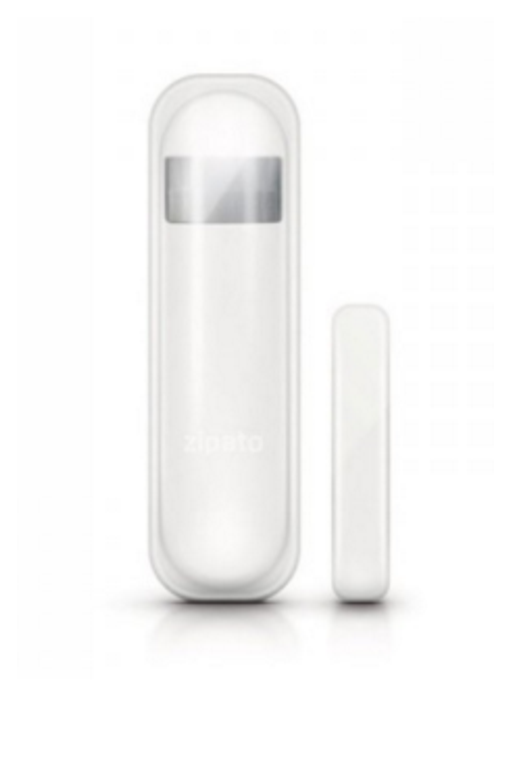
\includegraphics[width=.4\linewidth,keepaspectratio,angle=0]{figuras/Zipato.eps}
	\caption{Multisensor 4 em 1, Zipato.}
\end{minipage}\hfill
\begin{minipage}{.45\textwidth}
	\centering
	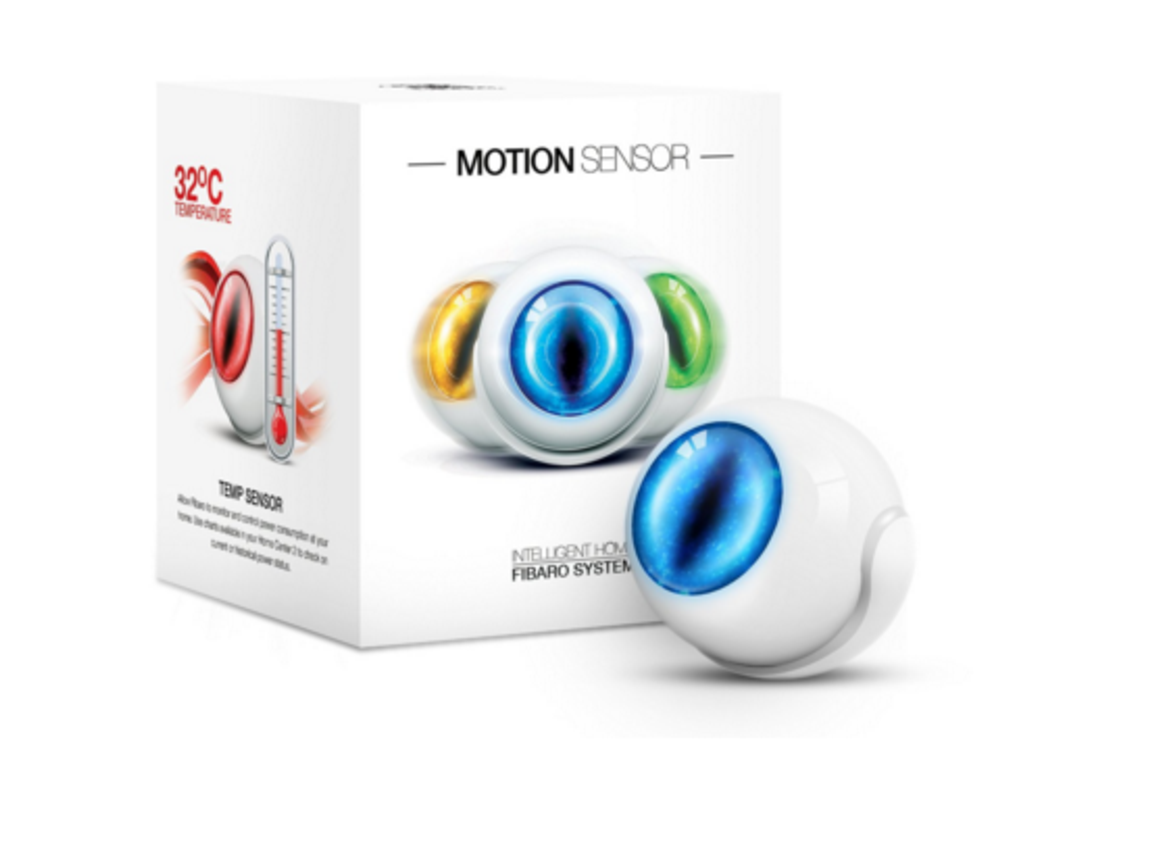
\includegraphics[width=.7\linewidth,keepaspectratio,angle=0]{figuras/Fibaro.eps}
	\caption{Sensor 2 em 1, Fibaro.}
\end{minipage}
\end{figure}

\begin{table}[H]
\centering
\begin{tabular}{|c|c|c|}
\hline 
\textbf{Fabricante} & \textbf{Zipato} & \textbf{Fibaro}\tabularnewline
\hline 
\hline 
\textbf{Modelo} & PH-PSM02 & FGMS-001\tabularnewline
\hline 
\textbf{Valor} & $R\$59,00$ & $R\$57,99$\tabularnewline
\hline 
\textbf{Ânguo de detecção} & 90\textsuperscript{o} & 90\textsuperscript{o}\tabularnewline
\hline 
\textbf{Alcance de detecção} & 8$\si{\meter}$ & 7$\si{\meter}$\tabularnewline
\hline 
\textbf{Faixa de medição \textsuperscript{o}C} & -10 a 70\textsuperscript{o}C & -20 a 100\textsuperscript{o}C\tabularnewline
\hline 
\textbf{Temperatura operação} & -10 a 40\textsuperscript{o}C & 0 a 40\textsuperscript{o}C\tabularnewline
\hline 
\textbf{Duração da bateria} & 2 anos & 2 anos\tabularnewline
\hline 
\end{tabular}
\caption{Características dos sensores de movimento e temperatura.}
\end{table}

	Nota-se, de acordo com a tabela, que a única diferença considerável, além da temperatura de funcionamento, é o alcance de detecção. Como a diferença de preço é bem pequena, o sensor escolhido foi o Zipato\cite{MovimentoZWave}, que tem alcance de 8m, 1m a mais que o concorrente.

	O sensor PH-PSM02 da Zipato, é projetado para atender à exigência de integrar 4 sensores em um único componente. Que são eles: Temperatura, Iluminação, Sensor de movimento por calor e Detecção de abertura ou fechamento de portas e janelas.

	Além disso este sensor é alimentado por bateria do tipo CR123A, que possui um custo aproximado de $R\$ 11,00$\cite{BateriaPanasonic}, e duração de 2 anos, ou seja, não interfere no consumo energético da casa.

\begin{itemize}
\item Custo total : $3\times$ \texteuro$59,00 =\ $\texteuro$177,00$

\item Quantidade: 1 (Sala de estar/jantar), 1 (Garagem); 1(Cozinha).

Notar que a quantidade de sensores está ligada à quantidade de acessos (entradas) da casa. Total de 3 sensores.

\item Consumo: Independente, 1 bateria do tipo CR123A.
\end{itemize}

\subsection{Ducha}

	Entre as opções de ducha o seguimento tem pouca inovação. As novidades ficam por conta do controle de fluxo e de temperatura digitalmente. Na pesquisa, buscou-se comparar entre as mais diferentes possíveis, então surgiu a comparação de uma ducha e um misturador:

\begin{figure}[H]
\centering
\begin{minipage}{.45\textwidth}
	\centering
	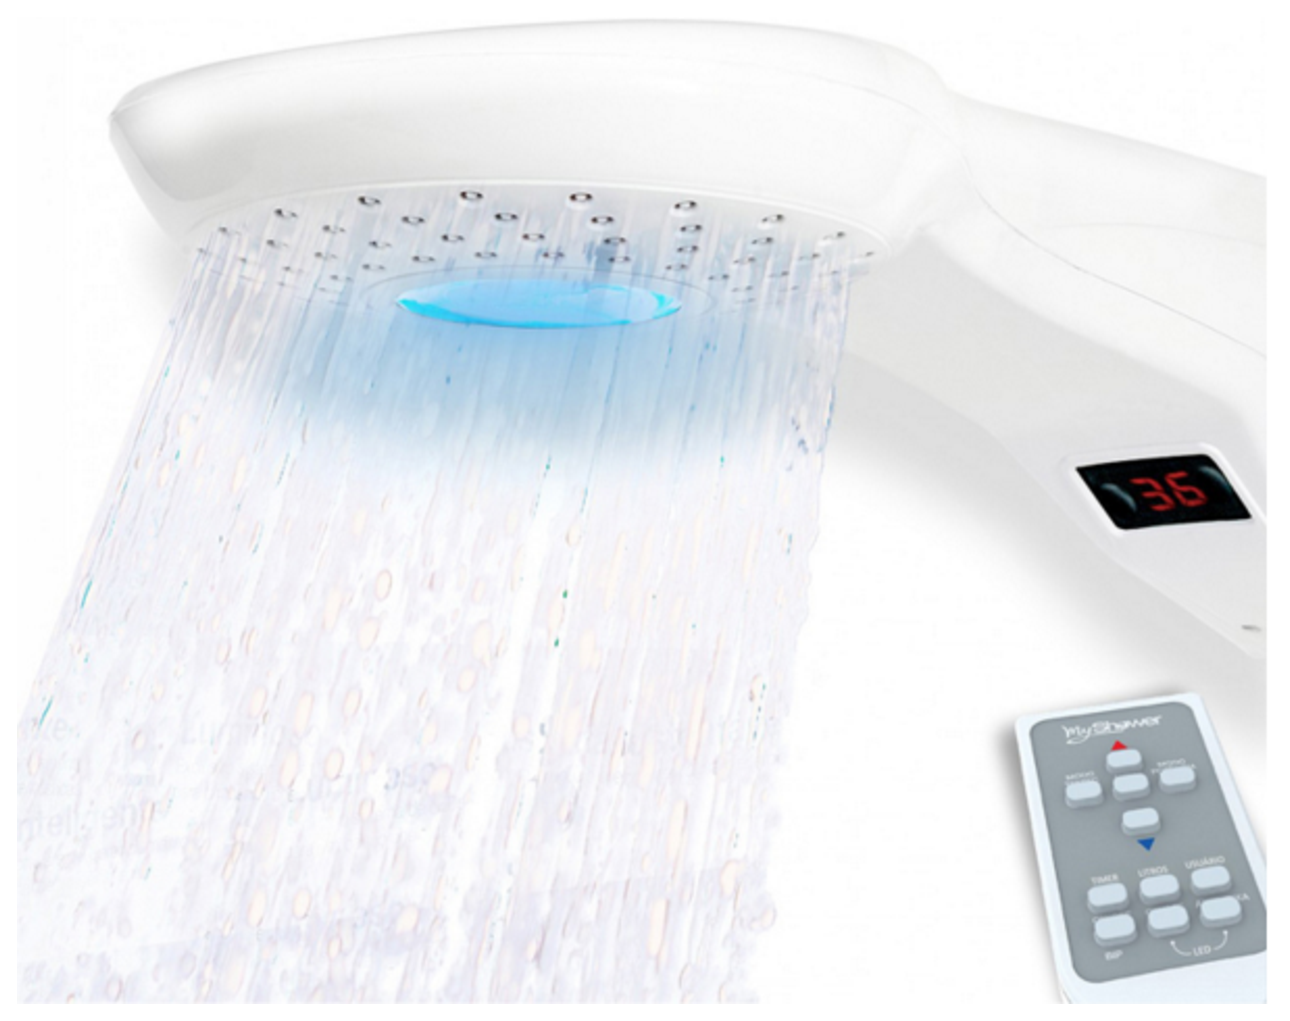
\includegraphics[width=.7\linewidth,keepaspectratio,angle=0]{figuras/MyShower.eps}
	\caption{Ducha Eletrônica Exatron Sensorial, MyShower.}
\end{minipage}\hfill
\begin{minipage}{.45\textwidth}
	\centering
	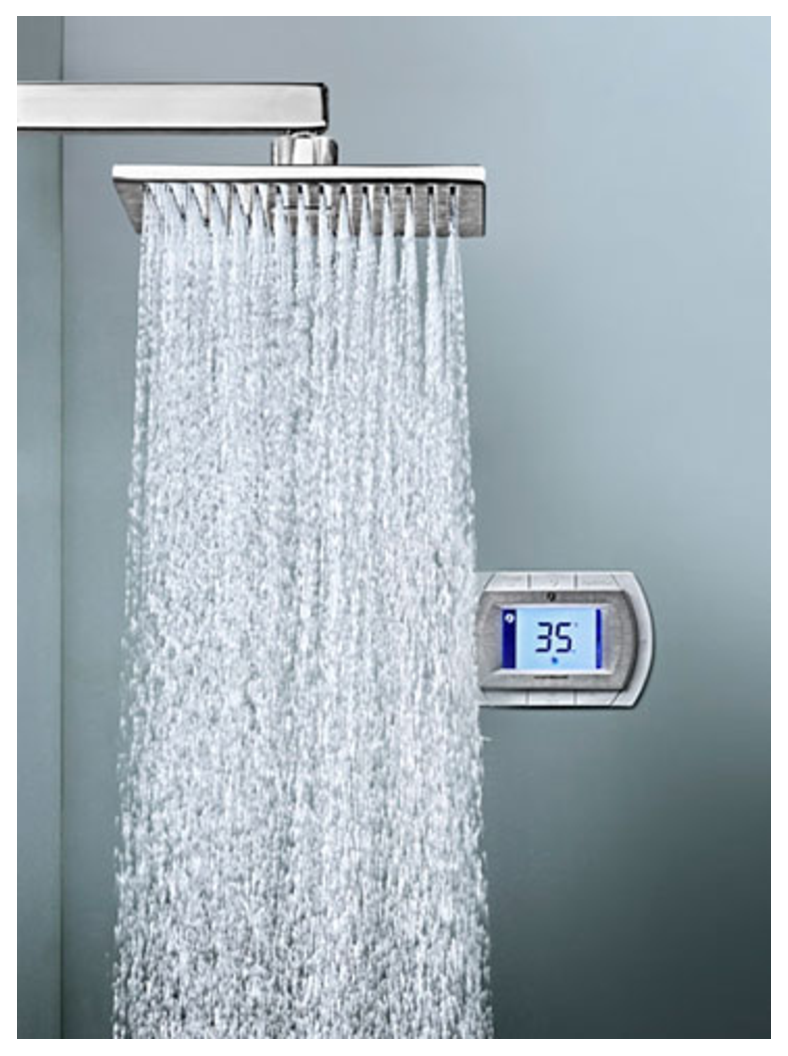
\includegraphics[width=.5\linewidth,keepaspectratio,angle=0]{figuras/Ihouse.eps}
	\caption{SmartShower com seu painel ao fundo, Ihouse.}
\end{minipage}
\end{figure}

\begin{table}[H]
\centering
\begin{tabular}{|c|c|c|}
\hline 
\textbf{Modelo} & \textbf{MyShower} & \textbf{SmartShower}\tabularnewline
\hline 
\hline 
\textbf{Potência} & 7500$\si{\watt}$ & 6$\si{\watt}$\tabularnewline
\hline 
\textbf{Pré aquecimento} & Não & sim\tabularnewline
\hline 
\textbf{Tipo} & Ducha & Misturador\tabularnewline
\hline 
\textbf{Consumo mín. mensal} & 30,6 $\tfrac{\si{\kilo\watt}}{\si{\hour}}$ & -\tabularnewline
\hline 
\textbf{Consumo máx. mensal} & 9,6 $\tfrac{\si{\kilo\watt}}{\si{\hour}}$ & -\tabularnewline
\hline 
\textbf{Pressão mín.} & 0.5 M. col. Água & -\tabularnewline
\hline 
\textbf{Pressão máx.} & 4,1 m.c.a. sem regulador & -\tabularnewline
\hline 
\textbf{Custo} & R\$ 439,12 & R\$ 9.818,19\tabularnewline
\hline 
\end{tabular}
\caption{Características das duchas selecionadas.}
\end{table}

Dentre as opções, as desvantagens do SmartShower\cite{SmartShoweriHouse} estão no valor e na necessidade de um aquecedor externo. Por outro lado, o MyShower\cite{MyShowertaQi} tem um custo acessível e aquecimento próprio, além de prezar pela economia de água, com sistema de redução de desperdício e nota ao fim do banho. Tem-se então uma disputa entre a economia de energia por parte do SmartShower e a economia de água por parte do MyShower. Como a energia é uma das prioridades do escopo do projeto foi escolhido o SmartShower em função de sua economia de 1250 vezes menos energia que o MyShower. Sendo assim, o sistema de banho da casa, um sistema quase que com consumo nulo ao final do mês.

\begin{itemize}
\item Custo: $3\times R\$ 9.818,19\ =\ R\$ 29.454,57.$
\item Quantidade: 3 chuveiros (Um para cada banheiro).
\item Consumo energético mensal: 0,36 KWh
\end{itemize}

	O cálculo do consumo do SmartShower foi feito, levando em consideração 4 moradores, onde cada morador usaria o SmartShower durante 15 minutos, duas vezes por dia, dessa forma o consumo foi obtido do seguinte modo: 

	\begin{equation} \label{consumo_energetico_mensal} \tag{e.q. consumo energético mensal}
	\begin{split}
	C_{onsumo} &= P_{otência}\times \dfrac{H_{oras}}{D_{ias}}\times D_{ias}\\
	C_{onsumo} &= 6 \si{\watt}\times 2\si{\hour}\times 30\\
	C_{onsumo} &= 0,36 \si{\kilo\watt\hour}
	\end{split}
	\end{equation}

\subsection{Sensor de fumaça}

	Dentre as opções do mercado, os detectores de fumaça eram todos muito próximos, em todas as características, se distinguindo apenas em temperatura de operação e custo. Dessa forma escolheu-se o sensor que possuía o menor custo. O sensor escolhido foi o da marca Vision Security\cite{FumacaZWave}.

	 Este detector usa a rede Z-Wave para comunicação e é projetado para detectar a fumaça que vem para a sua câmara de detecção, uma vez detectada, o alarme do detector de fumaça soará. Esse sensor possui uma sensibilidade de fumaça de $\tfrac{0.5\%}{ft}$ e uma faixa de operação de temperatura de $-10^oC$ à $60^oC$.

\begin{figure}[H]
\centering
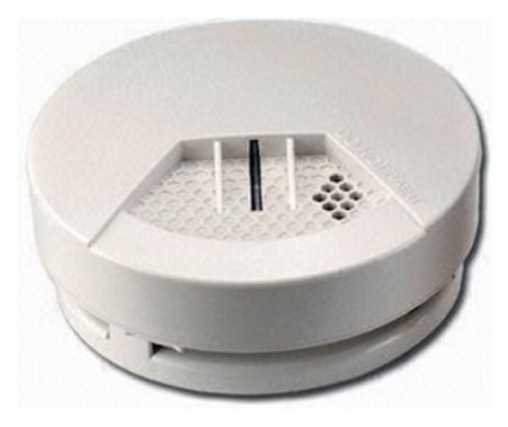
\includegraphics[width=.4\linewidth,keepaspectratio,angle=0]{figuras/VisioSecurity.eps}
\caption{Sensor de fumaça, ZS 6101 Visio Security.}
\end{figure}

\begin{itemize}
\item Custo: \texteuro58,68.
\item Quantidade: 1 (Casa de máquinas).
\item Consumo: Independente, 1 bateria do tipo CR123A. 
\end{itemize}

\subsection{Câmeras}
	
	Entre os sensores, as câmeras são as que exigem atenção especial e demandam tempo de pesquisa em alguns aspectos como transmissão de dados, qualidade da imagem e alcance. As opções encontradas foram 3 da marca Foscam:

\begin{table}[H]
\centering
\begin{tabular}{|c|c|c|c|}
\hline 
\textbf{Modelo} & \textbf{Fi - 9853} & \textbf{Fi - 9831} & \textbf{Fi - 8904}\tabularnewline
\hline 
\hline 
\textbf{Instalação} & Fixa & Móvel & Fixa\tabularnewline
\hline 
\textbf{Resolução} & 1280x720 & 1280x960 & 640x480\tabularnewline
\hline 
\textbf{Valor} & \texteuro104,49 & R\$ 1.130,90 & R\$ 1.000,00\tabularnewline
\hline 
\textbf{Alcance} & $50\si{\meter}$ & $8\si{\meter}$ no escuro & $15\si{\meter}$ no escuro\tabularnewline
\hline 
\textbf{Ângulo de alcance} & 70\textsuperscript{o} & 80\textsuperscript{o} & 50\textsuperscript{o}\tabularnewline
\hline 
\textbf{Liberdade} & - & 300\textsuperscript{o} H/ 120\textsuperscript{o} V & -\tabularnewline
\hline 
\end{tabular}
\caption{Características das câmeras encontradas.}
\end{table}

	As câmeras serão utilizadas 24 horas por dia no monitoramento da casa, visando uma melhor segurança para os moradores.

	Dentre os modelos disponíveis, a Fi-8904 chamou atenção pela resolução de menor qualidade, que resulta em maior facilidade para transmissão e pelo seu baixo custo. Além dela, a Fi-9831 teve a vantagem de ser móvel e motorizada, podendo cobrir uma área maior de vigilância. O preço é um pouco mais elevado, porém, devido à característica de se movimentar, menos unidades dela serão necessárias. Então a Fi-9853 foi dispensada e serão adquiridas unidades dos modelos Fi-9831 e Fi-8904.

	 O modelo Fi – 9831 possui sensor de luminosidade, ativando seus leds automaticamente de modo que seu alcance no escuro chegue a 8 metros, suporta cartões de memória (até 32GB) e possui entrada e saída de áudio.

\begin{figure}[H]
\centering
\begin{subfigure}{.45\textwidth}
	\centering
	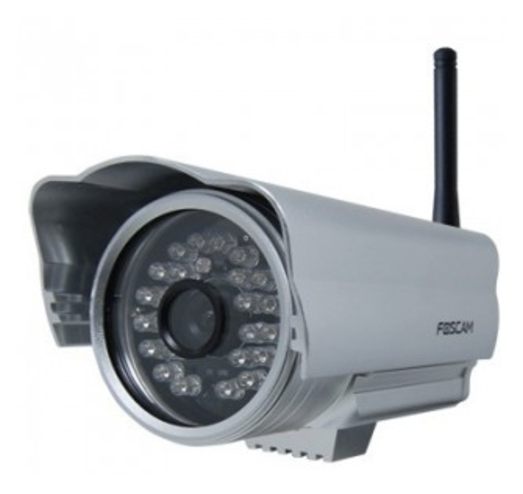
\includegraphics[width=.7\linewidth,keepaspectratio,angle=0]{figuras/camera1.eps}
\end{subfigure}\hfill
\begin{subfigure}{.45\textwidth}
	\centering
	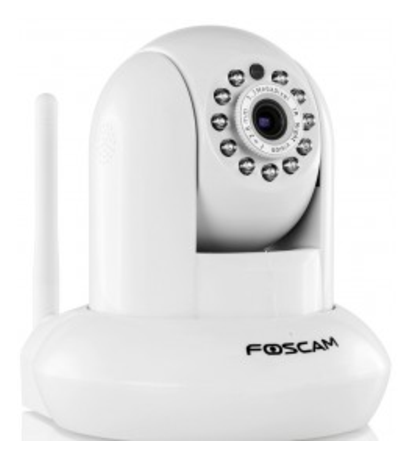
\includegraphics[width=.5\linewidth,keepaspectratio,angle=0]{figuras/camera2.eps}
\end{subfigure}
\caption{Câmeras utilizadas para monitoramento externo.}
\end{figure}

\begin{itemize}
\item Custo: $5\times R\$ 1.000 + 3\times R\$1.130,90\ =\ R\$ 8.392,70$.
\item Quantidade: 5 fixas e 3 móveis. Todas para vigilância exterior.
\item Consumo Fi-9831: $7.6 \si{\watt}$
\item Consumo Fi-8904: $14 \si{\watt}$
\item Consumo energético mensal\footnote{O consumo energético foi calculado de acordo com a equação \ref{consumo_energetico_mensal}}: $15.552 \si{\kilo\watt\hour}$
\end{itemize}

\subsection{Iluminação}

	Para definir a iluminação foi necessário, antes de tudo, entender quais os parâmetros de luz no ambiente. A medida de fluxo luminoso presente na maioria das lâmpadas é o Lúmen. Isso dá um padrão a ser seguido em critérios de luminescência. Por outro lado, para de definir a iluminação é determinado ambiente se utiliza o Lux, que é dado por Lúmem/m². Segundo a NBR 5412, que entrou em desuso em 2013 para ser substituída pela NBR 8995-1\cite{DisciplinasUTFPR}* existe um padrão específico para lâmpadas residenciais, conforme a tabela da página a seguir.

	Para escolher as lâmpadas, os parâmetros de influência em comportamento foram levados em conta. Ou seja, o projeto se importa em dar cores específicas para determinados cômodos de acordo com a sua função na casa. De maneira geral, cada cor remete a emoções e sensações diferentes \cite{InfluenciaGoi}. O amarelo, por exemplo, estimula o apetite e aumenta a concentração. Por outro lado, o azul aumenta a sensação de amplitude e o verde traz a sensação de bem-estar por estar em uma freqüência nem muito longa e nem muito curta. 

\begin{table}[H]
\centering
\begin{tabular}{|c|c|c|}
\hline 
\multicolumn{2}{|c|}{\textbf{Ambiente}} & \textbf{Lux}\parnote{Luminância mínima}\tabularnewline
\hline 
\hline 
\multirow{3}{*}{\textbf{Sala}} & \textbf{Luz Geral} & 50 - 100\tabularnewline
\cline{2-3} 
 & \textbf{Tarefa Rápidas} & 150\tabularnewline
\cline{2-3} 
 & \textbf{Ler, costurar} & 300\tabularnewline
\hline 
\multicolumn{2}{|c|}{\textbf{Sala de Jantar}} & 50 - 200\tabularnewline
\hline 
\multirow{2}{*}{\textbf{Dormitório}} & \textbf{Luz geral} & 50\tabularnewline
\cline{2-3} 
 & \textbf{Cabeceira} & 150\tabularnewline
\hline 
\multicolumn{2}{|c|}{\textbf{Cozinha}} & 300 - 500\tabularnewline
\hline 
\multirow{2}{*}{\textbf{Banheiro}} & \textbf{Luz geral} & 100\tabularnewline
\cline{2-3} 
 & \textbf{Luz do espelho} & 200\tabularnewline
\hline 
\multicolumn{2}{|c|}{\textbf{Hall}} & 150\tabularnewline
\hline 
\textbf{Escritório} & \textbf{Mesa de Trabalho} & 300 - 500\tabularnewline
\hline 
\multicolumn{2}{|c|}{\textbf{Garagem}} & 50\tabularnewline
\hline 
\end{tabular}
\parnotes
\caption{Descrição da quantidade de Lux indicada para cada cômodo.}
\end{table}

Para que o ambiente siga os critérios apresentados anteriormente, é necessário que a luzes se adaptem de acordo com a necessidade do proprietário, com esse intuito, foram escolhidas luzes no padrão RGB. As opções eram poucas:

\begin{table}[H]
\centering
\begin{tabular}{|c|c|c|}
\hline 
Fabricante & Aeotec & Zipato\tabularnewline
\hline 
\hline 
Custo & \texteuro59 & \texteuro69,9\tabularnewline
\hline 
Fluxo & 400lm & 850lm\tabularnewline
\hline 
Consumo & 6,7W & 9W\tabularnewline
\hline 
Vida útil & 50.000 & 50.000\tabularnewline
\hline 
Temp. Funcionamento & -40\textsuperscript{o}C a 50\textsuperscript{o}C & 0\textsuperscript{o}C a 40\textsuperscript{o}C\tabularnewline
\hline 
\end{tabular}
\caption{Lâmpadas RBG encontradas no mercado.}
\end{table}

	Foi escolhida a lâmpada da empresa Zipato pela proporção de lúmen/potência. Ou seja, com um gasto menor de energia, tem-se uma capacidade de iluminação quase dobrada. O contra seria a capacidade de operação em temperaturas de no máximo 40\textsuperscript{o}C, porém, como a temperatura máxima registrada no DF foi de 35,8\textsuperscript{o}C, registrada em 2008 \cite{2015ComG1} desde o início das medições em 1961, ainda existe uma margem segura para o seu funcionamento.

	Com a área de aproximadamente 76$\si{\meter}^2$, a sala precisará de 9 lâmpadas para luz geral e, sobre a área central, haverá mais um conjunto de mais 5 lâmpadas, já que a área é de 31,5$\si{\meter}^2$. 

	Já a sala de jogos, com seus 31$\si{\meter}^2$, precisará de 6 lâmpadas enquanto os quartos de 12$\si{\meter}^2$ precisarão de 1 lâmpada cada. O quarto de casal, entretanto, com 30$\si{\meter}^2$, precisará de 2 lâmpadas. Cada banheiro necessitará 2 lâmpadas, sendo que na casa existem 2, seria um total de 4 lâmpadas para os banheiros. Considerando o corredor e as salas pequenas, a casa necessitará de um \textbf{total de 32 lâmpadas}.

\begin{figure}[H]
\centering
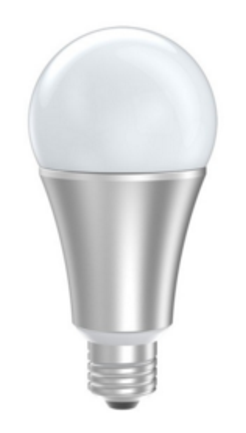
\includegraphics[width=.2\linewidth,keepaspectratio,angle=0]{figuras/zipato.eps}
\caption{Lâmpadas utilizadas para iluminação interna, fabricante Zipato.}
\end{figure}

\begin{itemize}
\item Custo: $32\times $\texteuro$ 69,90 =\ $\texteuro$ 2.236,80$
\item Consumo: $9\times 32 = 288\si{\watt}$
\item Consumo energético mensal\footnote{O consumo energético foi calculado de acordo com a equação \ref{consumo_energetico_mensal}} $69,12 \si{\kilo\watt\hour}$
\end{itemize}

\subsection{HomeTroller S6}

\begin{figure}[H]
\centering
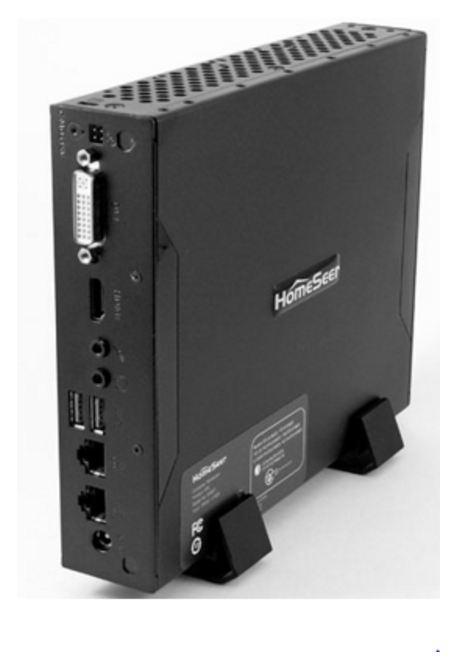
\includegraphics[width=.35\linewidth,keepaspectratio,angle=0]{figuras/hometroller.eps}
\caption{Aparelho HomeTroller S6 da HomeSeer.}
\end{figure}

	De acordo com os controladores da Homeseer, este se apresenta mais completo, com um melhor processador, possuindo entradas e saídas de áudio. 

\subsubsection{Descrição}

	HomeTroller Série 6 é um controlador de automação residencial que combina a confiabilidade e a simplicidade de um controlador do tipo painel com o poder e a flexibilidade de um controlador baseado em software. Oferece reconhecimento de voz, integração com telefone permitindo gerenciar remotamente o aparelho, texto para processamento de voz, e-mail e acesso remoto protegido \cite{HomeSeerHomeTroller}.

	O sistema é gerido através de qualquer navegador web, permitindo facilmente adicionar/alterar horários, ou solucionar problemas \cite{2009AutomacaoMarilia}. HomeTroller S6 PRO consome apenas 15 watts de potência em operação normal e inclui o software HS3Touch Designer para que o usuário possa criar seus próprios projetos de acordo com as suas preferências \cite{HomeSeerHomeTroller}.

\subsubsection{Especificações}
\begin{itemize}
\item Software de controle imbutido: HomeSeer HS3PRO
\item Sistema operacional: Windows 7 Incorporado
\item Processador: 1.8 GHz dual core Intel Celeron CPU
\item Memória: 4 GB RAM
\item Armazenamento: 32 GB SSD
\item Portas: (2) RS232 (6), USB, Microfone in/Line out, (2) 10/100/1000 LAN, DVI, HDMI
\item Consumo de energia: Menos de 15 watts (nominal)
\item Dimensões: $8$\textquotedbl$\times6.5$\textquotedbl$\times1,5$\textquotedbl.
\item Fonte de alimentação: 120-240V Universal, 50 / 60Hz (plug EUA)
\item Certificações: UL, CE, RoHS
\item Valor: $1,199.95$ Dólares 
\end{itemize}

\subsubsection{O que está incluído}
\begin{itemize}
\item HomeTroller S6 W / incorporado HS3PRO
\item HS3Touch Designer
\item Todos os Drivers HomeSeer Branded Software (plug-ins)
\item Pés de fixação
\item Suporte de parede
\item Cabo Ethernet
\item Adaptador elétrico universal
\item Cabo de alimentação (com plug EUA)
\end{itemize}

\subsubsection{Tecnologias Suportadas}

\subsubsubsection{Z-Wave}
\textbf{Características:}
\begin{itemize}
\item \textbf{Empresa : Zensys}
\item Tecnologia totalmente sem fio
\item Não tem largura da banda suficiente para transmissão de áudio ou vídeo \cite{PrincipaisTeruelFilho}.
\item Comunicação de mão dupla – envio e recebimento de sinal.
\item Pouco consumo de energia
\item Pode-se adquirir novos dispositivos com chip Z-Wave e conectá-los sem qualquer complicação.
\item Permite 232 dispositivos colocados a uma distância máxima de 30m \cite{PrincipaisTeruelFilho}.
\item O chip Z-Wave é responsável pela escolha da melhor rota para o transporte de dados para outros dispositivos.
\item Solução interessante principalmente para residências já construídas por não precisar alterar a parte da construção.
\item Inviável para sistemas com mais de 30 dispositivos, se tratando de recursos financeiros \cite{PrincipaisTeruelFilho}.
\end{itemize}

\subsubsubsection{Insteon}
\textbf{Características:}
\begin{itemize}
\item Empresa: SmartHome
\item Usa a rede elétrica para o transporte de dados entre os dispositivos.
\item Cada equipamento tem um endereço para o qual o sinal é direcionado.
\item Protocolo de comunicação não permite desvio ou perda de sinal por oscilações na rede elétrica \cite{PrincipaisTeruelFilho}.
\item Usa protocolo de comunicação plug-and-play de mão dupla (envio e recebimento de sinal).
\item Transporte de dados pode se dar por cabeamento ou radiofrequência.
\item Radiofrequência da tecnologia Insteon trabalha em uma frequência entre 902-924 MHz, atinge uma distância de 150 pés \cite{2005BeyondDritsas}.
\item Não é tão segura, interferências podem não permitir que o sinal atinja seu destino com eficiência (como de um aparelho de micro-ondas).
\item Pode ser transmitido por rede elétrica com capacidade de funcionar com 110 ou 220 volts \cite{2005BeyondDritsas}.
\end{itemize}

\subsubsubsection{X10}
\textbf{Características:}
\begin{itemize}
\item Desenvolvida nos anos 70 pela Pico Eletronics..
\item Umas das primeiras tecnologias da área.
\item Limitada a operar apenas com funções simples(liga/desliga e dimerização de luzes).
\item Comunicação entre transmissores e receptores por meio da rede elétrica\cite{2004ResidenciasBolzani}.
\item Protocolo de comunicação de mão única - apenas envia.
\item Produtos relativamente baratos.
\item Fácil instalação e aplicação.
\end{itemize}

\subsubsubsection{UPB (Universal Powerline Bus)}
\textbf{Características:}
\begin{itemize}
\item Comunicação via rede Elétrica.
\item Não necessita de novos cabeamentos, pois usa a rede elétrica existente. 
\item Possui transmissão de até quase 2 km \cite{TecnologiaConverge}.
\item Pulsos de 40 Volts. Frequências de 4 a 40 KHz( Baixa frequência não afetar outros dispositivos) \cite{TecnologiaConverge}.
\item Comunicação bidirecional.
\item Pode ser utilizada na presença de outras tecnologias.
\end{itemize}

\subsubsubsection{PLC-BUS (Power Line Communication Bus)}
\textbf{Características:}
\begin{itemize}
\item Usa a rede elétrica existente.
\item Principais características: Comunicação digital totalmente encriptada e a bidirecionalidade \cite{PLCMKTI}.
\item Pode utilizar a radiofrequência para distribuição na rede eléctrica sob a forma de código PLC-BUS transformados para atuarem sobre os diversos componentes do sistema.
\item A encriptação do sinal permite a utilização de até um máximo de 64.000 endereços numa mesma instalação\cite{PLCMKTI}. 
\item Após a observação das tecnologias utilizadas pelo HomeTroller S6, foi escolhida a tecnologia Z-Wave por apresentar comunicação sem fio o que melhor possibilita a implementação numa residência já construída
\end{itemize}

\subsection{Motores}

	Quando há a necessidade de se controlar um motor com o protocolo Z-Wave, no mercado encontra-se disponíveis controladores, mas não os motores. Janelas têm módulos específicos de controle, o que torna a tarefa de controlá-las um pouco mais simples. As opções se diferem em dois tipos:

\begin{table}
\centering
\begin{tabular}{|c|c|c|}
\hline 
\textbf{Fabricante} & \textbf{Fibaro} & \textbf{Somfy}\tabularnewline
\hline 
\hline 
\textbf{Capacidade} & 1 motor & 16 motores\tabularnewline
\hline 
\textbf{Alcance} & 30 m & -\tabularnewline
\hline 
\textbf{Consumo} & <0,8W & -\tabularnewline
\hline 
\textbf{Custo} & US\$ 74,59 & US\$ 450,00\tabularnewline
\hline 
\end{tabular}\caption{Comparação entre os controladores de janela.}
\end{table}

	A casa terá um total de 7 janelas que precisarão de cortinas controladas. Dessa forma, quando se calcula o custo de se utilizar o sistema Fibaro\cite{Manualaitesas}\cite{Valoraitesas} o prejuízo sai em torno de 450 – (6 x 74,59) = US\$ 2,46 Entretanto, por falta de informações técnicas e de instalação por parte do sistema da Somfy \cite{Caracteristicasaitesas}, o modelo Fibaro será escolhido. 

	Para abrir torneiras, no caso da irrigação, existe o controlador GR-105 da Smart Home, que alcança ¼ de de giro pode ser conectado diretamente na válvula da torneira. Apenas a smart home faz esse tipo de atuador, então ele será escolhido pela facilidade de manuseio, sem precisar interferir no sistema hidráulico da casa. Consome apenas 12W por hora de funcionamento.

\begin{figure}[H]
\centering
\begin{minipage}{.45\textwidth}
	\centering
	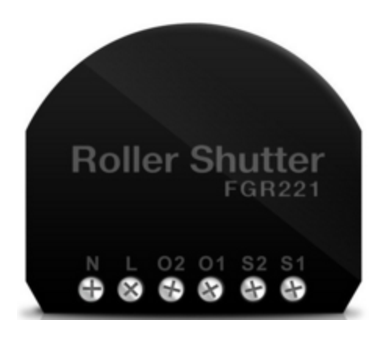
\includegraphics[width=.7\linewidth,keepaspectratio,angle=0]{figuras/rollershutter.eps}
	\caption{Modelo de controlador de cortinas da Fibaro.}
\end{minipage}\hfill
\begin{minipage}{.45\textwidth}
	\centering
	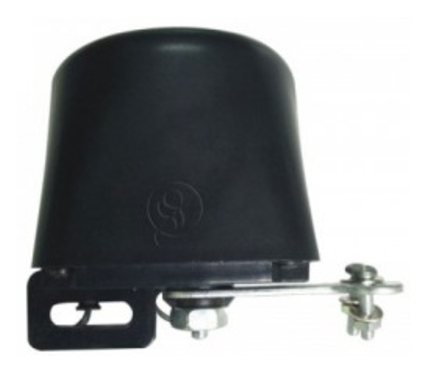
\includegraphics[width=.7\linewidth,keepaspectratio,angle=0]{figuras/controlador_adaptavel.eps}
	\caption{Controlador adaptável de \nicefrac{1}{4} de giro.}
\end{minipage}
\end{figure}

\begin{itemize}
\item Quantidade: 10 controladores de cortinas e 1 abridor de registro.
\item Custo: $US\$ 10\times74,59 + $\texteuro$ 79,95$
\item Consumo: $8\si{\watt} + 12\si{\watt}$

\end{itemize}

\subsection{Comunicação IR}

	Alguns produtos não tem comunicação direta com a central Z-Wave, dessa forma se faz necessária a integração a partir de extensores infra-vermelho. Estes extensores recebem ordens de dispositivos Z-Wave e as enviam em IV, podendo controlar desde os condicionadores de ar até o equipamento de som. Só um extensor foi encontrado: o Modelo ZXT-120 \cite{ExtensorZWave}. 

\begin{figure}[H]
\centering
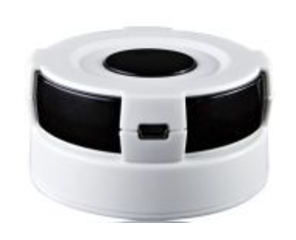
\includegraphics[width=.7\linewidth,keepaspectratio,angle=0]{figuras/extensor.eps}
\caption{Extensor Modelo ZXT-120}
\end{figure}

\begin{itemize}
\item Quantidade:

1 para cada equipamento controlado por infravermelho. Parte-se do pressuposto que a casa tem TV, DVD e Home theater.

\item Custo:$ 3\times81,00 =\ \texteuro 243,00$
\item Consumo: independente, 3 pilhas AAA.
\end{itemize}

\subsection{Posição dos Sensores}

A posição dos sensores será estabelecida de acordo com a necessidade da casa e obedecendo às características exigidas pelo manual. Dessa forma, deve-se lembrar que os sensores de movimento não podem ser instalados em áreas externas, as câmeras tem ângulo de alcance de 30o e uma distância máximo de 30m, isso deve ser levado em conta na hora de fazer a obertura de monitoramento da casa. Como os equipamentos tem alcance de 30m não será necessário o uso de repetidores, já que o lote tem justamente esse tamanho. O mapa de sensores ficou da seguinte maneira:

\begin{figure}[H]
  \begin{center}
	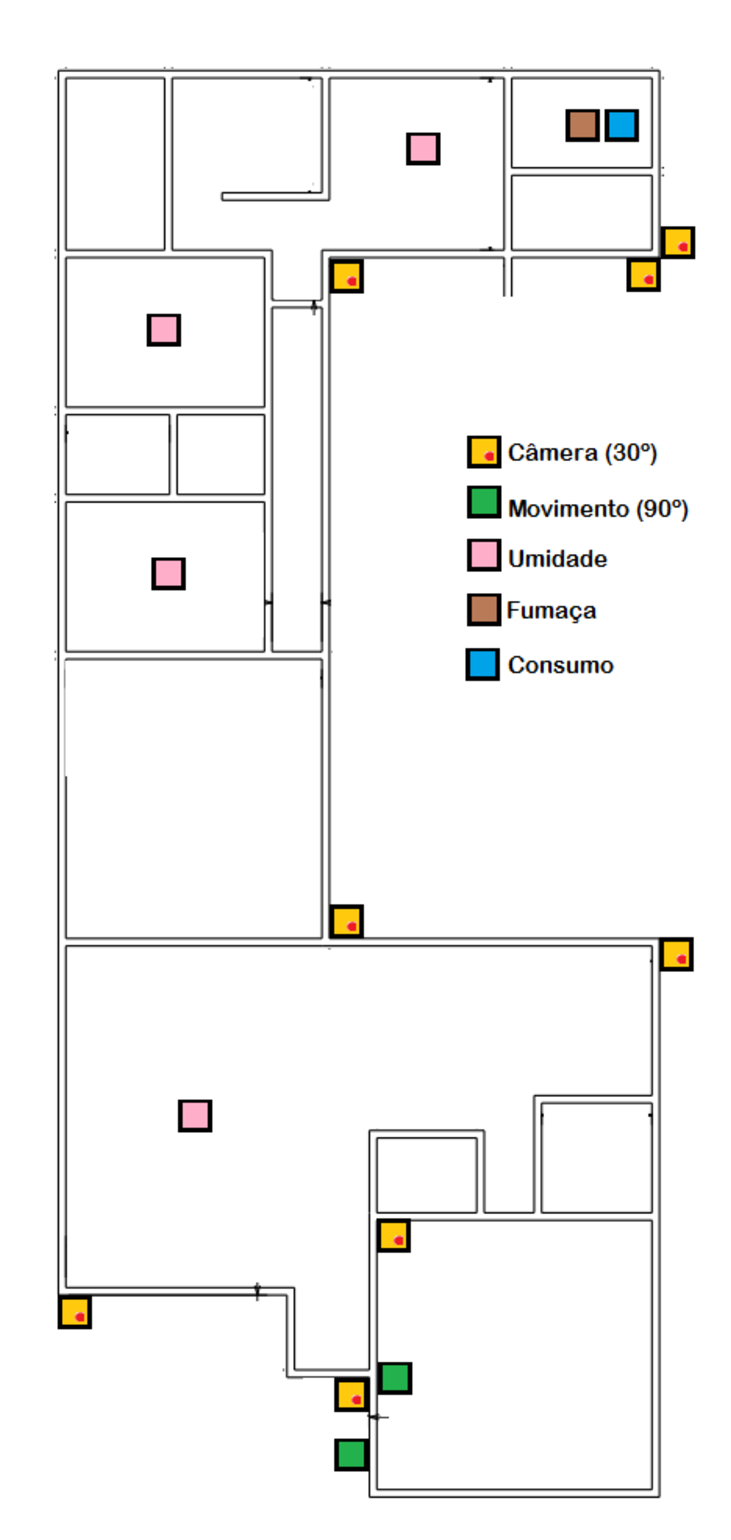
\includegraphics[keepaspectratio,scale=0.6,angle=270]{figuras/posicao.eps}
	\caption{Posição dos sensores na casa}
  \end{center}
\end{figure}

\subsection{Custos totais e viabilidade do projeto.}

	Os equipamentos foram escolhidos de tal forma que os usuários disponham de um sistema com facilidade de operação, simplicidade de comandos, e que tais equipamentos atendam todas as demandas necessárias, mas não apenas isso, a viabilidade econômica também foi levada em consideração.
	
	Como decidido e justificado, a compra dos softwares para gerenciamento da Green Home se dará por meio da empresa Home Seer, onde iremos usar a plataforma de comunicação Z-Wave, de forma que para que não aja percas na comunicação e para que a interação software –hardware aconteça com qualidade, o principal pré-requisito para a compra dos equipamentos e sensores é que utilizem a tecnologia de comunicação Z-Wave.


*Foram adotados os valores de 4,14 para o dólar e 4,70 para o euro, pois de acordo com o site UOL Economias \cite{UolDolar}\cite{UolEuro}, esses foram as maiores cotações em 1 ano para as respectivas moedas em relação ao real. 

%%%%%%%%%%%%%%%%%%%%%%%%%%%%%%%%%%%%%%%%%%%%%%%%%%%%%%%%%%%%%%%%%%%%%%%%%%%%%%%
%%%%%%%%%%%%%%%%%%%%%%%%%%%%%%%% Falta Tabela %%%%%%%%%%%%%%%%%%%%%%%%%%%%%%%%
%%%%%%%%%%%%%%%%%%%%%%%%%%%%%%%%%%%%%%%%%%%%%%%%%%%%%%%%%%%%%%%%%%%%%%%%%%%%%%%


	Assim como foi previamente estabelecido, o controlador escolhido foi o HomeTroller S6 PRO, sua compra se dará pela Homeseer com valor de 1.199,95 dólares \cite{HomeSeerHomeTroller}, a compra do sensor de movimento e temperatura se dará na Zipato, uma empresa localizada na Croácia e do detector de fumaça da empresa Vision Security será efetuada por meio de uma loja online de produtos Z-Wave localizada em Portugal \cite{ProdutosZwave}. As câmeras serão da fabricante Foscam, e sua compra se dará por meio da loja virtual do fabricante \cite{LojaFoscam}.
	Optou-se pelo SmartSHower pertencente a empresa Ihouse, mas que é vendida pela empresa IpSum Smart no Brasil. O pré-orçamento deste item está disponível no anexo 1. 

